\documentclass[border={-7pt -5pt -5pt -3pt}]{standalone}
\usepackage{tikz}
\usetikzlibrary{decorations.pathreplacing,
  arrows,
  calc,
  decorations.pathmorphing,
  decorations.pathreplacing,
  decorations.markings,
  fadings,
  positioning,
  shapes,
  3d
}
\begin{document}
\begin{tikzpicture}
  \node at (0, 0) {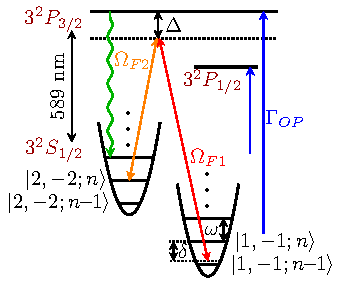
\includegraphics[height=4.5cm]{schematics.pdf}};
  \node at (3.75, 0.4) {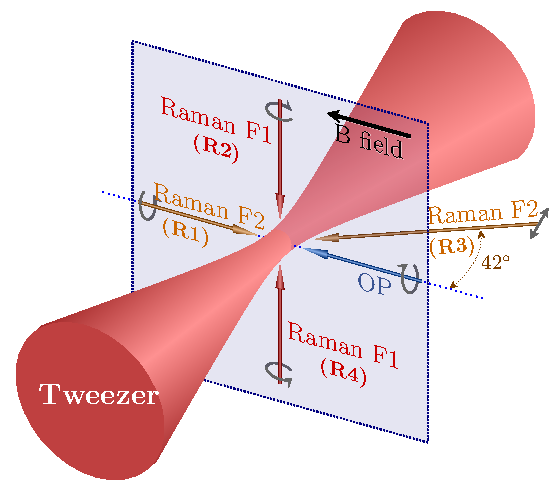
\includegraphics[height=3.65cm]{geometry.pdf}};
  \node at (10.6, 0) {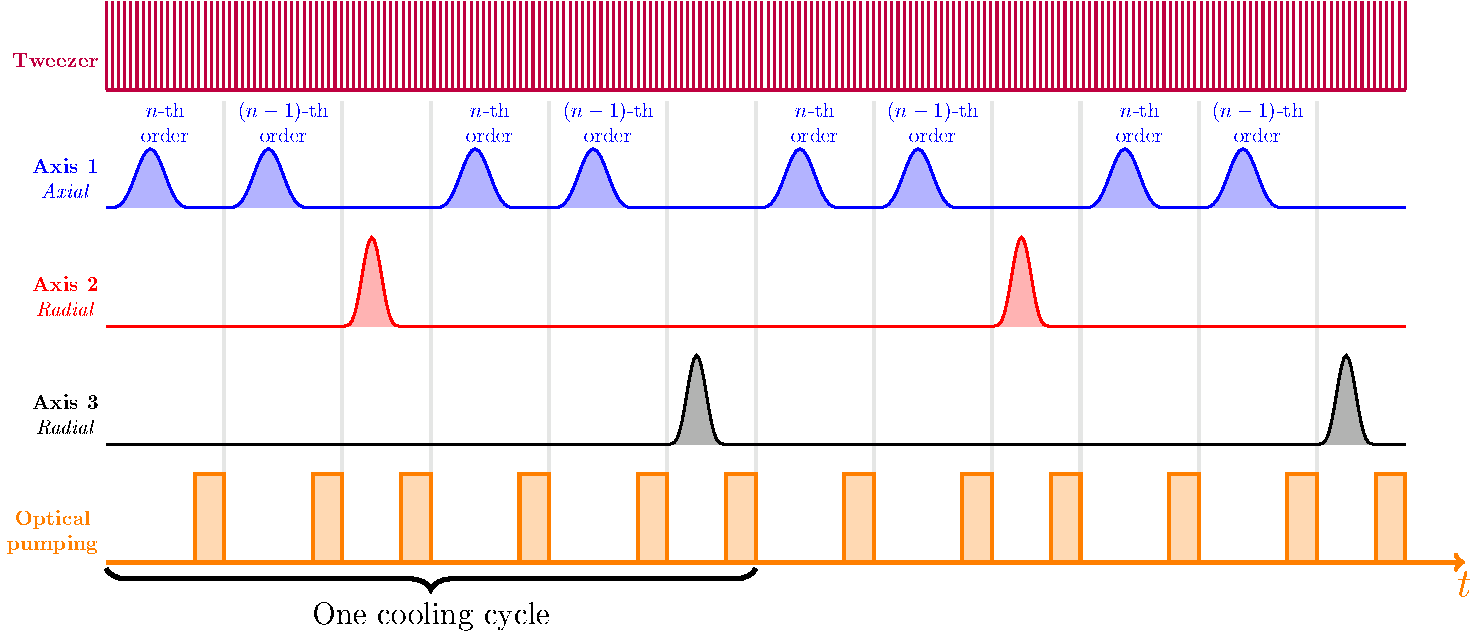
\includegraphics[height=4.5cm]{sequence.pdf}};
  \node at (-1.4, -1.8) {(A)};
  \node at (3.15, -1.8) {(B)};
  \node at (6.2, -1.8) {(C)};
\end{tikzpicture}
\end{document}
